\newpage
\subsection{Temporary repository for synergy suggestions}

\begin{itemize}
    \item EWK phase transition: LISA
    \item Fine structure constant measurements: AMO
\end{itemize}

\subsection{Temporary repository for cross references to be made with other sections}

\begin{itemize}
    \item need the accelerators to be defined in accelerator part by Lenny and Caterina.
    \item need the hierarchy problem to be discussed in introductory chapter by Gian
    \item reference to BSM section for DM and naturalness
    \item reference to flavor for CP
\end{itemize}

%\bibliography{\main/section1/bib/section}

\subsection{Things that could be put into an appendix or that are useful to keep while finalizing our chapter}
\begin{table}[]
    \centering
    \caption{Number of $Z$ bosons and $W$-pairs for each of the colliders at various $\sqrt{s}$ values. The LEP and SLC numbers reflect the numbers actually produced.
    \label{tab:ewkprogramme}
    \KE{LEP: 4 detectors, each with integrated luminosity of about 200 pb$^{-1}$
SLC: 600,000 measured, 350,000 in last two years.
LEP: numbers for W-pairs include production at threshold and above.}
\BH{CLIC 380, information by email from Philipp Rohloff assumes 50:50 split between +80\% and -80\% polarisation.}}
\begin{tabular}{l r|c c|cr|c|c}
         Collider                          & $\sqrt{s}$    & $\Delta t$ (yr) & $\int\cal{L}$d$t$ (\iab)& Particle & Number & Pol. & default plan \\\hline
         LEP\cite{ALEPH:2005ab}            & $\sim M_Z$    & 7 & $0.8\times 10^{-3}$ & Z-boson & $1.7\times 10^7$ & no & yes \\
         SLD\cite{ALEPH:2005ab}            & $\sim M_Z$    & 6 & ? & Z-boson & $6\times 10^5$ & yes & yes \\ 
         \FCCee\cite{Abada:2019zxq} & $\sim M_Z$ & 4 & $150$ & Z-boson & $3\times 10^{12}$ & no & yes \\
         \CEPC\cite{CEPCStudyGroup:2018ghi} & $\sim M_Z$    & 2  & $16$  & Z-boson &$3\times 10^{11}$ & no & yes\\ 
         \ILC\cite{ILCZ}                    & $\sim M_Z$    & 1-3  & $0.1$ & Z-boson & $4.9\times 10^9$ & yes & no \\
         \CLIC\cite{CLICZ}                  & $\sim M_Z$    & few  & $0.1$ & Z-boson & $5\times 10^9$ & yes & no \\ 
         \ILC\cite{ILCZ}                    & $250$ GeV     & 11  & $2$ & Z-boson & $1.1\times 10^8$ & yes & yes \\
         \CLIC\cite{CLICZ}                  & $380$~GeV     & 8 & $1$ & Z-boson & $5\times 10^6$ & yes & yes \\\hline
         LEP\cite{Schael:2013ita}          & $\gtrsim 2M_W$& 5 & $3\times 10^{-3}$ & W-pairs & $5\times 10^4$ & no & yes \\
         \FCCee\cite{Abada:2019zxq}    & $\sim 2M_W$   & 2 & $12$ & W-pairs & $1\times 10^6$ & no & yes \\
         \CEPC\cite{CEPCStudyGroup:2018ghi} & $\sim 2M_W$   & 1  & $2.6$ & W-pairs & $1.5\times 10^7$ & no &yes\\
         \CEPC\cite{CEPCStudyGroup:2018ghi} & $240$~GeV     & 7 & $5.6$ & W-pairs & $9.5\times 10^7$ & no & yes\\
         \FCCee\cite{Abada:2019zxq}    & $240$~GeV     & 4 & $5$ & W-pairs & $8.5\times 10^7$ & no & yes\\
         \ILC\cite{Fujii:2017vwa}           & $250$~GeV     & 11 & 2 & W-pairs & $3.4\times 10^7$ & yes & yes\\
         \CLIC                              & $380$~GeV     & 8 & 1 & W-pairs& $1.3\times 10^7$ & yes & yes\\
    \end{tabular}
\end{table}

\begin{table}[htbp]
    \centering
    \caption{Higgs coupling measurements from ATLAS~\cite{atlashcomb2}, using between $36.1$ and $79.8$~fb$^{-1}$ for most analyses, and CMS~\cite{cmshcomb2}, using $35.9$~fb$^{-1}$ for all analyses\label{tab:higgsnow}. For the ATLAS $\kappa_t$ result only the allowed values with $\kappa_t>0$ are shown. The \HLLHC projections are also shown based on Ref.~\cite{deBlas:2019rxi}. \BH{Removed table from main text as we now have a nice plot containing the information.}
    \label{higgsnow}
    }
    \begin{tabular}{c|r|r|r}
    \hline
    parameter & ATLAS & CMS & \HLLHC\\\hline\hline
       $\kappa_Z$, $\kappa_V\leq 1$ & $> 0.87$ at 95\% CL & $-0.87 \pm 0.09$& $> 0.987$ at 95\% CL\\
       $\kappa_W$, $\kappa_V\leq 1$ & $> 0.85$ at 95\% CL & $-1.00^{+0.09}_{-0.00}$& $> 0.983$ at 95\% CL\\
       $\kappa_b$  & $0.88 \pm 0.13$ & $0.91^{+0.17}_{-0.16}$ & $\pm 0.026$\\
       $\kappa_t$  & $[0.93,1.24]$ at 68\% CL & $1.02^{+0.19}_{-0.15}$ &$\pm 0.028$\\
       $\kappa_\tau$  & $0.97 \pm 0.13$ & $0.93\pm 0.13$ & $\pm 0.016$\\
       $\kappa_g$  & $1.01^{+0.13}_{-0.11}$ & $1.16^{+0.18}_{-0.13}$ & $\pm 0.022$\\
       $\kappa_\gamma$  & $0.98 \pm 0.07$ & $0.96 \pm 0.09$ & $\pm 0.017$\\
       $\kappa_\mu$  & n.a. & $0.72 ^{+0.50}_{-0.72}$ & $\pm 0.044$\\
$B(H\to \textrm{inv.})$ & $<0.30$ at 95\% CL & $<0.22$ at 95\% CL & $<0.019$ at 95\% CL\\
$B(H\to \textrm{undet.})$ & $<0.22$ at 95\% CL & $<0.38$ at 95\% CL & $<0.041$ at 95\% CL\\
\hline
    \end{tabular}
\end{table}


\begin{figure}[!ht]
\centering
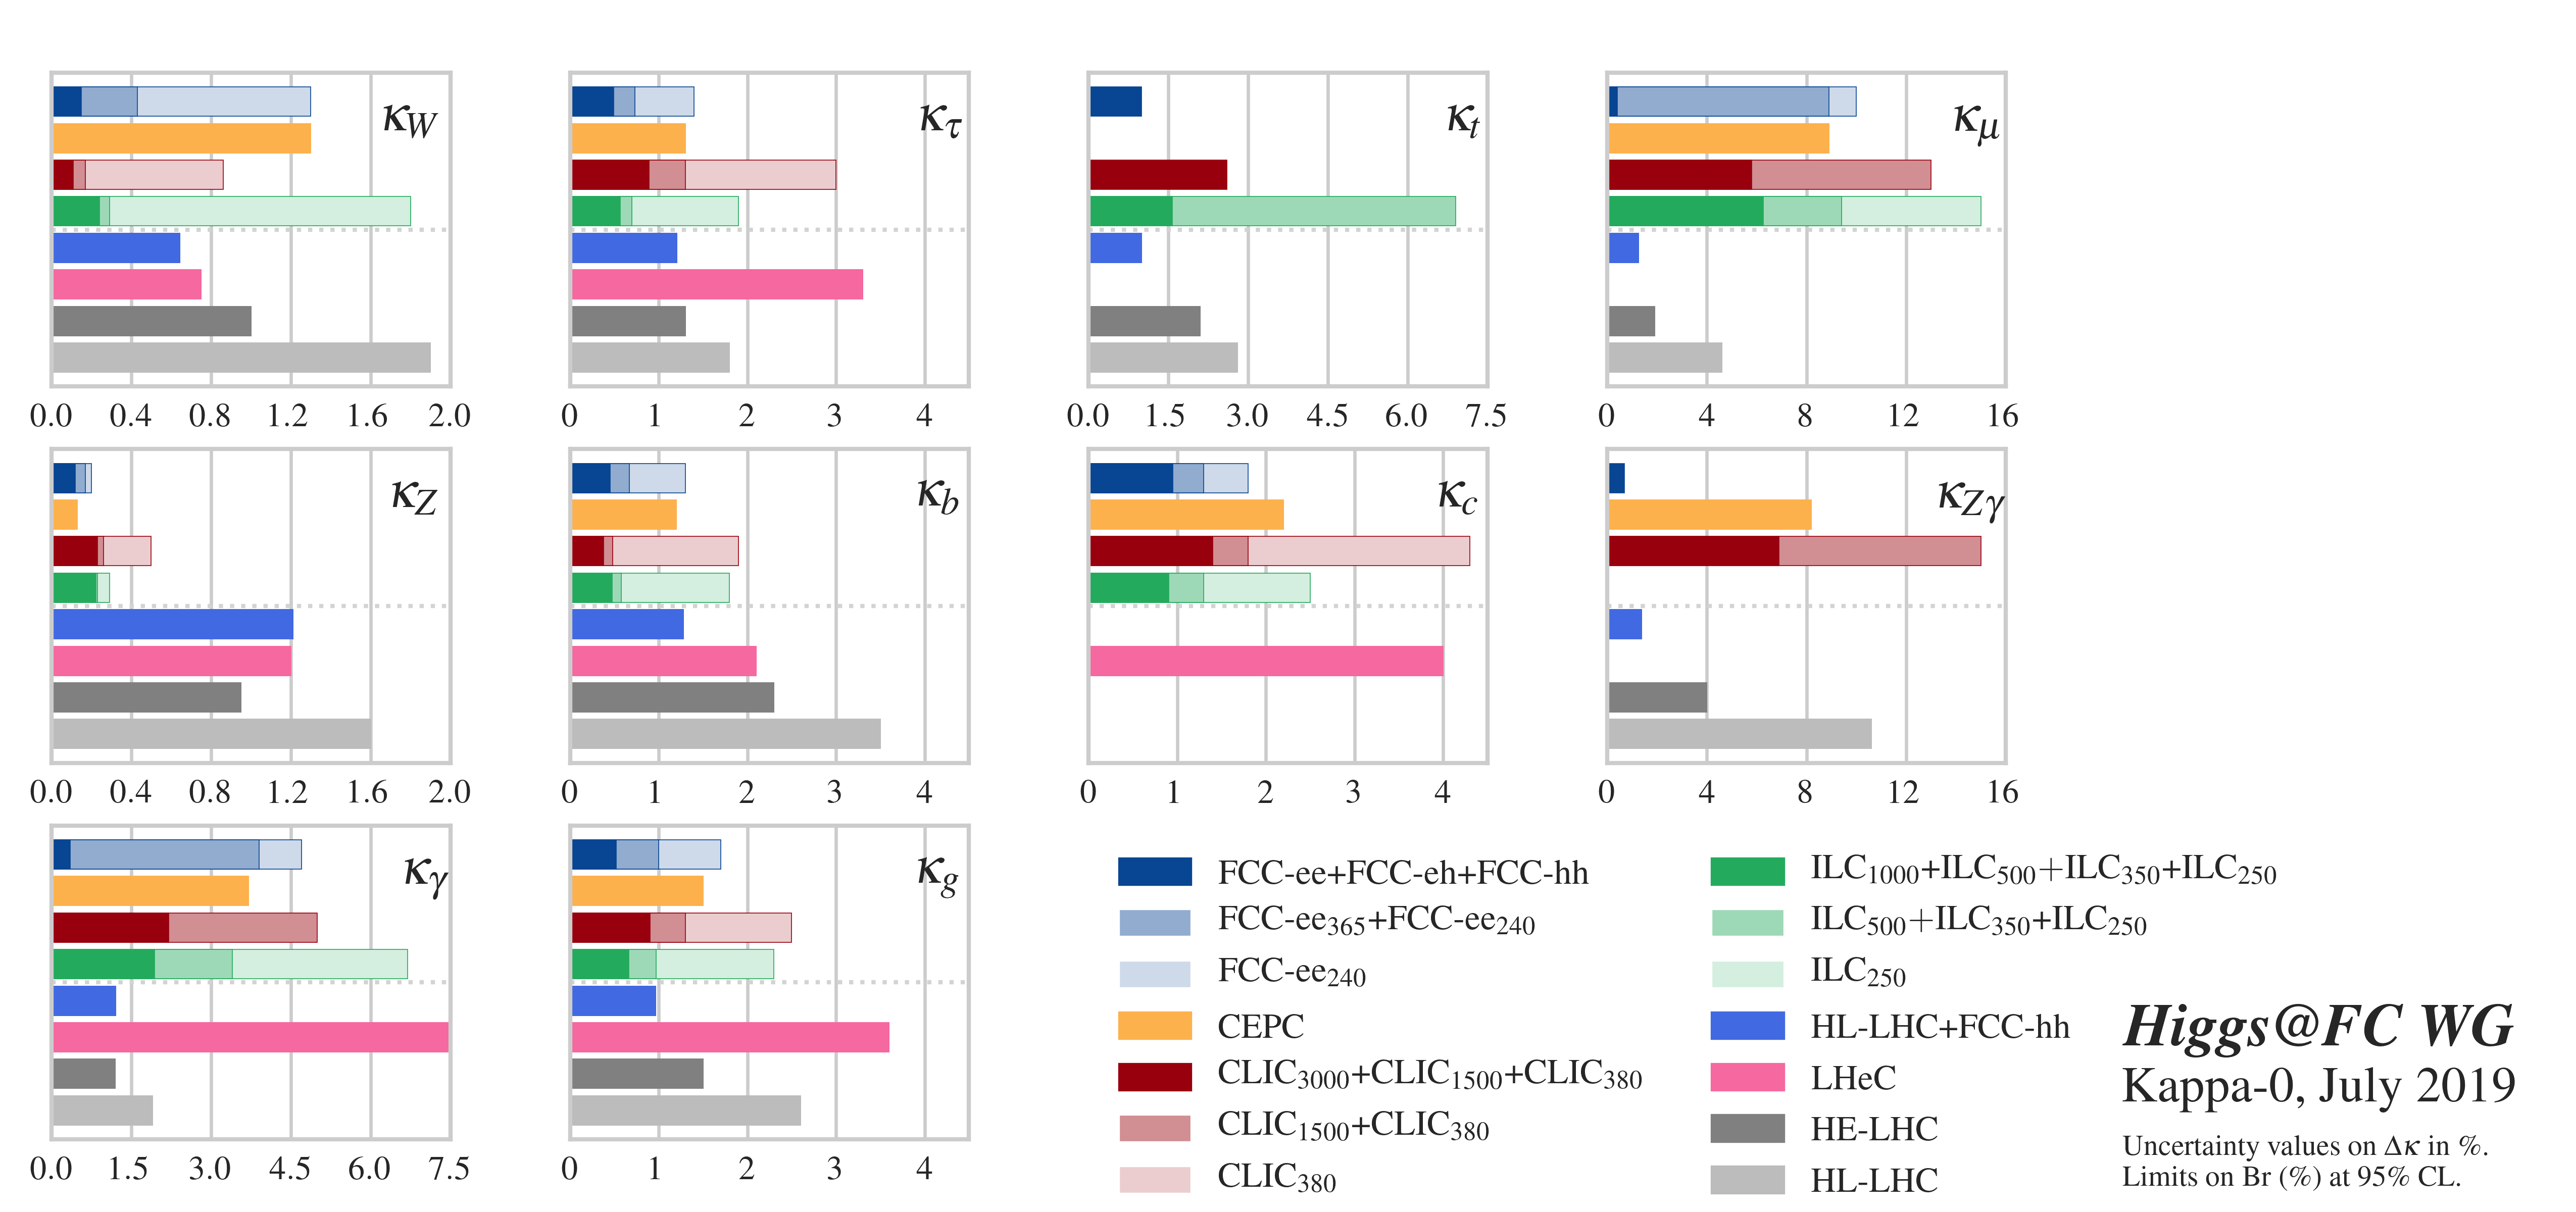
\includegraphics[width=.8\linewidth]{\main/ewksection/img/Kappa0WithNewColumns}
\caption{\label{fig:hkappa0new}
Plot of kappa-0 with \FCChh only and \ILC1000 included.
}
\end{figure}

